\documentclass[a4paper]{article}

\input{style/ch_xelatex.tex}
\input{style/scala.tex}

\lstset{numbers=left,
basicstyle=\tiny,
numberstyle=\tiny,
keywordstyle=\color{blue!70},
commentstyle=\color{red!50!green!50!blue!50},
frame=single, rulesepcolor=\color{red!20!green!20!blue!20}
}

\graphicspath{{fig/}{fig/generated/}}
\usepackage[fontset=none]{ctex}
\usepackage{graphicx}
\usepackage{booktabs}
\usepackage{multirow}
\usepackage{float}
\usepackage{geometry}
\usepackage{fancyhdr}
\usepackage{hyperref}
\usepackage{subfigure}
\usepackage{lastpage}

\setCJKmainfont{PingFang SC}
\setCJKsansfont{Heiti SC}
\setCJKmonofont{PingFang SC}
\setCJKfamilyfont{zhkai}{PingFang SC}
\newcommand{\kaishu}{\CJKfamily{zhkai}}

\geometry{a4paper,left=2.3cm,right=2.3cm,top=2.7cm,bottom=2.7cm}
\pagestyle{fancy}
\lhead{\kaishu \leftmark}
\rhead{\kaishu 深度学习及应用（高阶课）实验报告}
\lfoot{}
\cfoot{\thepage}
\rfoot{}
\renewcommand{\headrulewidth}{0.1pt}
\renewcommand{\footrulewidth}{0pt}
\setlength{\textfloatsep}{8mm}
\renewcommand{\today}{\number\year 年 \number\month 月 \number\day 日}

\begin{document}
\pagenumbering{gobble}
\renewcommand{\contentsname}{目\ 录}
\renewcommand{\refname}{参考文献}
\renewcommand{\figurename}{图}
\renewcommand{\tablename}{表}

\begin{titlepage}
    \begin{center}
    
\includegraphics[width=0.8\textwidth]{NKU.png}\\[1cm]
    \vspace{20mm}
		\textbf{\huge\textbf{\kaishu{计算机学院}}}\\[0.5cm]
		\textbf{\huge{\kaishu{深度学习及应用（高阶课）实验报告}}}\\[2.3cm]
		\textbf{\Huge\textbf{\kaishu{Seq2Seq 翻译实验}}}

		\vspace{\fill}
    \textsc{\LARGE \kaishu 姓名\ :\ 林晖鹏}\\[0.5cm]
    \textsc{\LARGE \kaishu 学号\ :\ 2312966}\\[0.5cm]
    \textsc{\LARGE \kaishu 专业\ :\ 计算机科学与技术}\\[0.5cm]

    \vfill
    {\Large \today}
    \end{center}
\end{titlepage}

\clearpage
\tableofcontents
\newpage

\renewcommand{\thefigure}{\thesection{}.\arabic{figure}}
\pagenumbering{arabic}
\setcounter{page}{1}
\cfoot{\thepage\ of \pageref{LastPage}}

\section{实验目的}
实验围绕基于注意力机制的 Seq2Seq 翻译模型展开，主要完成以下几个方面的内容：
\begin{enumerate}
    \item 实现纯 RNN 解码器的 Seq2Seq 基线模型；
    \item 实现 Bahdanau attention 与 Luong attention，并与纯 RNN Seq2Seq 进行对比；
    \item 观察引入注意力机制后，对翻译精度、整句匹配率、BLEU、训练时间与推理时间的影响；
    \item 进一步实现 Scheduled Sampling 作为扩展实验，观察其对注意力模型的影响。
\end{enumerate}

\section{实验设置}
\subsection{数据集与任务}
实验使用英法平行语料 \texttt{eng-fra.txt}，该数据与 PyTorch 官方 Seq2Seq 教程保持一致，原始来源为 Tatoeba / ManyThings 整理的英法双语句对。数据文件中每一行对应一组平行句，格式为“英文 + 制表符 + 法文”。在预处理阶段，沿用教程中的基本筛选方式，即先将文本统一转成小写并做 ASCII 归一化，再保留长度较短的句对，并进一步保留目标英文句以 \texttt{i am / he is / she is / you are / we are / they are} 等前缀开头的样本。经过上述处理后，最终保留下来的句对数量为 10522，其中训练集约 8417 条，验证集约 1052 条，测试集约 1053 条。任务为法译英，即输入法语句子，输出对应的英语翻译结果。

\subsection{统一实验设置}
为了保证不同模型之间的实验结果具有可比性，主实验统一采用 Adam 优化器，并固定 hidden size = 128、层数 = 1、epoch = 200、batch size = 512。考虑到不同模型对学习率较为敏感，因此先对候选学习率集合 $\{0.003, 0.002, 0.001, 0.0005, 0.0003\}$ 进行搜索，再使用验证集最佳准确率对应的学习率作为正式训练配置。

PyTorch 官方 Seq2Seq 教程在训练过程中提供了 teacher forcing 开关，因此这里也保留这一设置。主实验统一将 teacher forcing 比例固定为 0.5，一方面利用真实目标词帮助模型在训练前期稳定收敛，另一方面也使模型有一部分机会接触自身预测结果。在此基础上，扩展实验进一步引入 inverse sigmoid 形式的 Scheduled Sampling\cite{bengio2015scheduled}，并分别在 Bahdanau attention 与 Luong attention 上进行对比，用于考察动态 teacher forcing 策略对模型性能的影响。

\subsection{评价指标}
实验主要记录以下几类指标：
\begin{itemize}
    \item \textbf{loss}：对所有非 PAD 位置计算交叉熵损失；
    \item \textbf{token accuracy}：按词统计正确率；
    \item \textbf{exact match}：整句完全一致时计为正确；
    \item \textbf{BLEU}：用于衡量翻译 n-gram 匹配质量\cite{papineni2002bleu}；
\end{itemize}

\section{模型结构设计}
\subsection{纯 RNN Seq2Seq}
基线模型采用经典的 Encoder-Decoder 结构\cite{sutskever2014sequence}。其中编码器使用 GRU 将输入法语句子编码成隐藏状态，解码器则依赖编码器最终隐藏状态逐步生成英语句子。该结构实现简单，便于作为对照模型使用；但它需要将整句信息压缩到固定维度的向量中，因此在句子稍长时容易出现信息表达不足的问题。

\subsection{Bahdanau Attention}
Bahdanau attention\cite{bahdanau2014neural} 在每一个解码步都利用当前解码状态与编码器各时刻输出之间的关系进行加性打分，并通过 softmax 得到注意力权重。这样一来，解码器在生成当前目标词时不再只依赖单个固定向量，而是能够动态关注输入句子的不同位置，从而缓解信息瓶颈问题。

\subsection{Luong Attention}
Luong attention\cite{luong2015effective} 采用乘性对齐方式，先得到当前解码步的隐藏表示，再与编码器输出进行匹配并生成上下文向量。由于老师给出的实验要求中并没有强制指定这一方法，因此这里是在自学 Seq2Seq 与注意力机制相关资料时，额外了解到 Luong attention，并将其引入作为 Bahdanau attention 之外的另一种注意力实现进行对比。Luong 论文中还给出了 \texttt{dot}、\texttt{general} 和 \texttt{concat} 三种常见打分方式。这里在主实验中选取综合表现最好的 \texttt{concat} 版本作为 Luong attention 的代表，与 Bahdanau attention 和纯 RNN Seq2Seq 进行对比；在补充实验中，再对 \texttt{dot}、\texttt{general} 和 \texttt{concat} 三种打分方式做进一步比较，用来说明注意力打分函数设计对翻译结果的影响。

\subsection{Scheduled Sampling}
Scheduled Sampling\cite{bengio2015scheduled} 旨在缓解 teacher forcing 带来的训练阶段与推理阶段输入不一致问题。训练时模型并不总是接收真实目标词，而是按照预定策略逐步增加“使用模型自身预测作为下一步输入”的比例。这里将其作为注意力模型的扩展实验，分别在 Bahdanau attention 与 Luong attention 分支上进行对比，用来分析训练策略的变化能否进一步改善翻译表现。

\subsection{网络结构打印结果}
为便于报告引用，三种主模型对应的完整打印结果已单独整理到 \texttt{code/model\_prints/} 目录下，正文中仅保留结构摘要如下。

\begin{minipage}[t]{0.40\textwidth}
\textbf{Seq2Seq-RNN}
\begin{lstlisting}
Seq2SeqRNN(
  (encoder): EncoderRNN(
    Embedding(4343,128)
    Dropout(0.1)
    GRU(128,128)
  )
  (decoder): DecoderRNN(
    Embedding(2804,128)
    Dropout(0.1)
    GRU(128,128)
    Linear(128,2804)
  )
)
\end{lstlisting}
\end{minipage}\hfill
\begin{minipage}[t]{0.40\textwidth}
\textbf{Seq2Seq-Bahdanau}
\begin{lstlisting}
Seq2SeqAttention(
  (encoder): EncoderRNN(
    Embedding(4343,128)
    Dropout(0.1)
    GRU(128,128)
  )
  (decoder): AttnDecoderRNN(
    Embedding(2804,128)
    BahdanauAttention(
      query/key/score
    )
    GRU(256,128)
    Linear(128,2804)
  )
)
\end{lstlisting}
\end{minipage}

\textbf{Seq2Seq-Luong}
\begin{lstlisting}
Seq2SeqLuong(
  (encoder): EncoderRNN(
    Embedding(4343,128)
    Dropout(0.1)
    GRU(128,128)
  )
  (decoder): LuongDecoderRNN(
    Embedding(2804,128)
    LuongAttention(concat)
    GRU(128,128)
    Linear(256,128)
    Linear(128,2804)
  )
)
\end{lstlisting}

\section{实验结果分析}
\subsection{主实验：三种模型对比}
三个主模型在正式训练配置下的核心结果如表\ref{tab:main_results}所示。

\begin{table}[H]
    \centering
    \small
    \resizebox{\textwidth}{!}{
    \begin{tabular}{lcccccc}
    \toprule
    模型 & 学习率 & Test Acc/\% & Test Exact/\% & Test BLEU($\times 100$) & 训练时长/s & FLOPs \\
    \midrule
    Seq2Seq-RNN & 0.002 & 66.55 & 26.50 & 44.36 & \textbf{142.37} & \textbf{1.594M} \\
    Seq2Seq-Bahdanau & 0.003 & 71.87 & 31.15 & 51.08 & 181.26 & 1.603M \\
    Seq2Seq-Luong & 0.002 & \textbf{72.73} & \textbf{31.72} & \textbf{51.77} & 178.28 & \textbf{1.594M} \\
    \bottomrule
    \end{tabular}
    }
    \caption{三种主模型的测试结果对比}
    \label{tab:main_results}
\end{table}

从表\ref{tab:main_results}可以看出：加入注意力机制后，模型性能明显优于纯 RNN Seq2Seq。引入注意力机制的方法相对基线在 Test Acc、Test Exact 和 BLEU 上都有较明显提升，说明注意力机制能够有效改善翻译质量。

\begin{figure}[H]
    \centering
    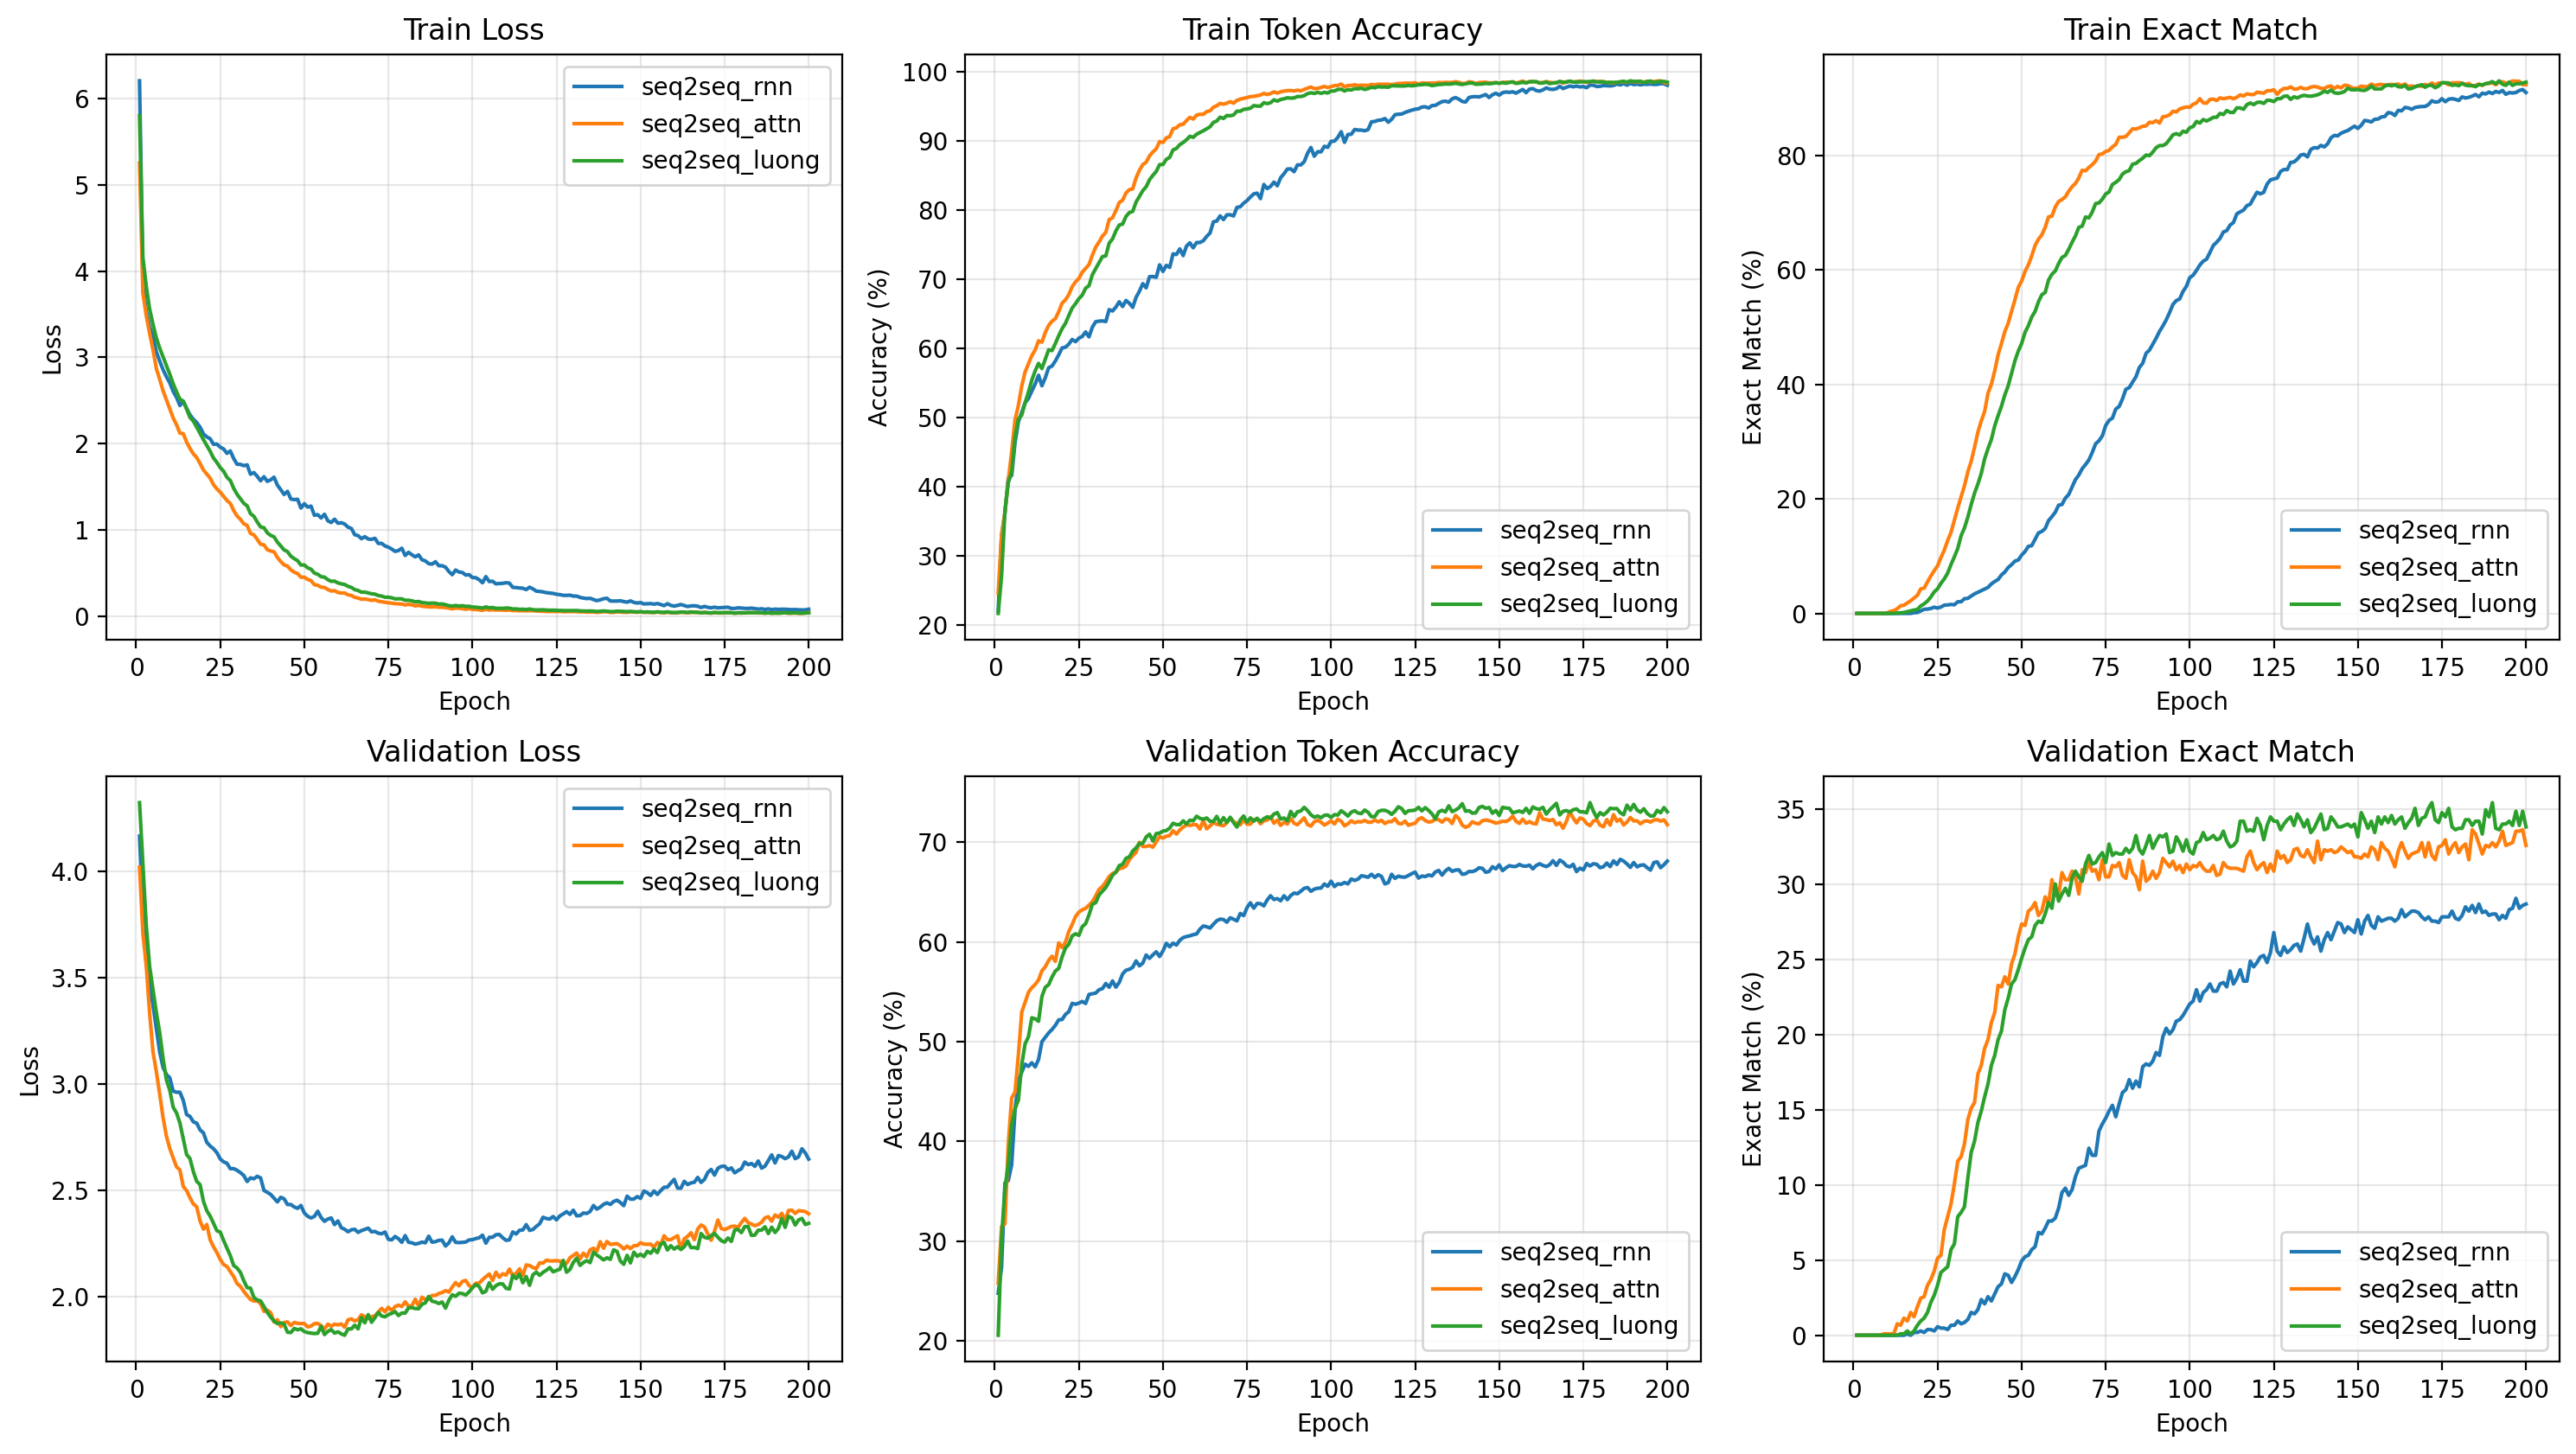
\includegraphics[width=0.9\textwidth]{fig/generated/best_run_val_curves.png}
    \caption{三种主模型的训练集与验证集曲线对比}
    \label{fig:curves}
\end{figure}


\subsection{训练过程曲线}
图\ref{fig:curves} 展示了三个主模型在训练集与验证集上的 loss、token accuracy 与 exact match 曲线。整体来看，纯 RNN 基线在训练后期的训练指标提升更快，但验证指标提升有限，说明其更容易出现过拟合；两种 attention 模型的验证曲线整体更平稳，其中 Luong concat 在验证集上的 accuracy 与 exact match 均保持在较高水平。

从训练曲线与最终指标可以进一步看出，不同模型在优化稳定性与泛化能力上呈现出不同特点。纯 RNN Seq2Seq 在训练集上收敛较快，但验证集性能明显落后，说明仅依赖固定上下文向量时更容易受到信息瓶颈限制。Bahdanau attention 在加入加性对齐之后，验证性能已有明显改善；而当前使用 concat scoring 的 Luong 版本在验证集和测试集上的综合表现进一步提升，说明注意力打分方式的设计同样会影响最终翻译效果。

另外，从图中还可以观察到，后期训练集指标明显高于验证集指标。例如某些模型在训练集上 token accuracy 已超过 95\%，但验证集只有 70\% 左右。这里需要说明的是，这种差距不能直接全部归因于严重过拟合。训练阶段在计算 loss、token accuracy 与 exact match 时，会以一定概率使用真实的上一个目标词作为下一步输入；而验证与测试阶段采用完全自回归的生成方式，模型只能使用自己上一步的预测结果继续解码。因此，训练指标与验证指标本身就不是完全同一口径，验证结果通常会明显低于训练结果。在此基础上，当前数据规模较小、训练轮数较多，后期确实仍存在一定过拟合现象，但它并不是训练集和验证集差距较大的唯一或者主要原因。


\subsection{长度分桶分析}
为了进一步分析注意力机制对不同句长样本的影响，除了保留长度分桶统计外，还按真实句长逐点统计了测试集上的 Exact Match 与 BLEU。图\ref{fig:lengthwise_plot} 给出了三种主模型在不同输入长度下的变化趋势。

\begin{figure}[H]
    \centering
    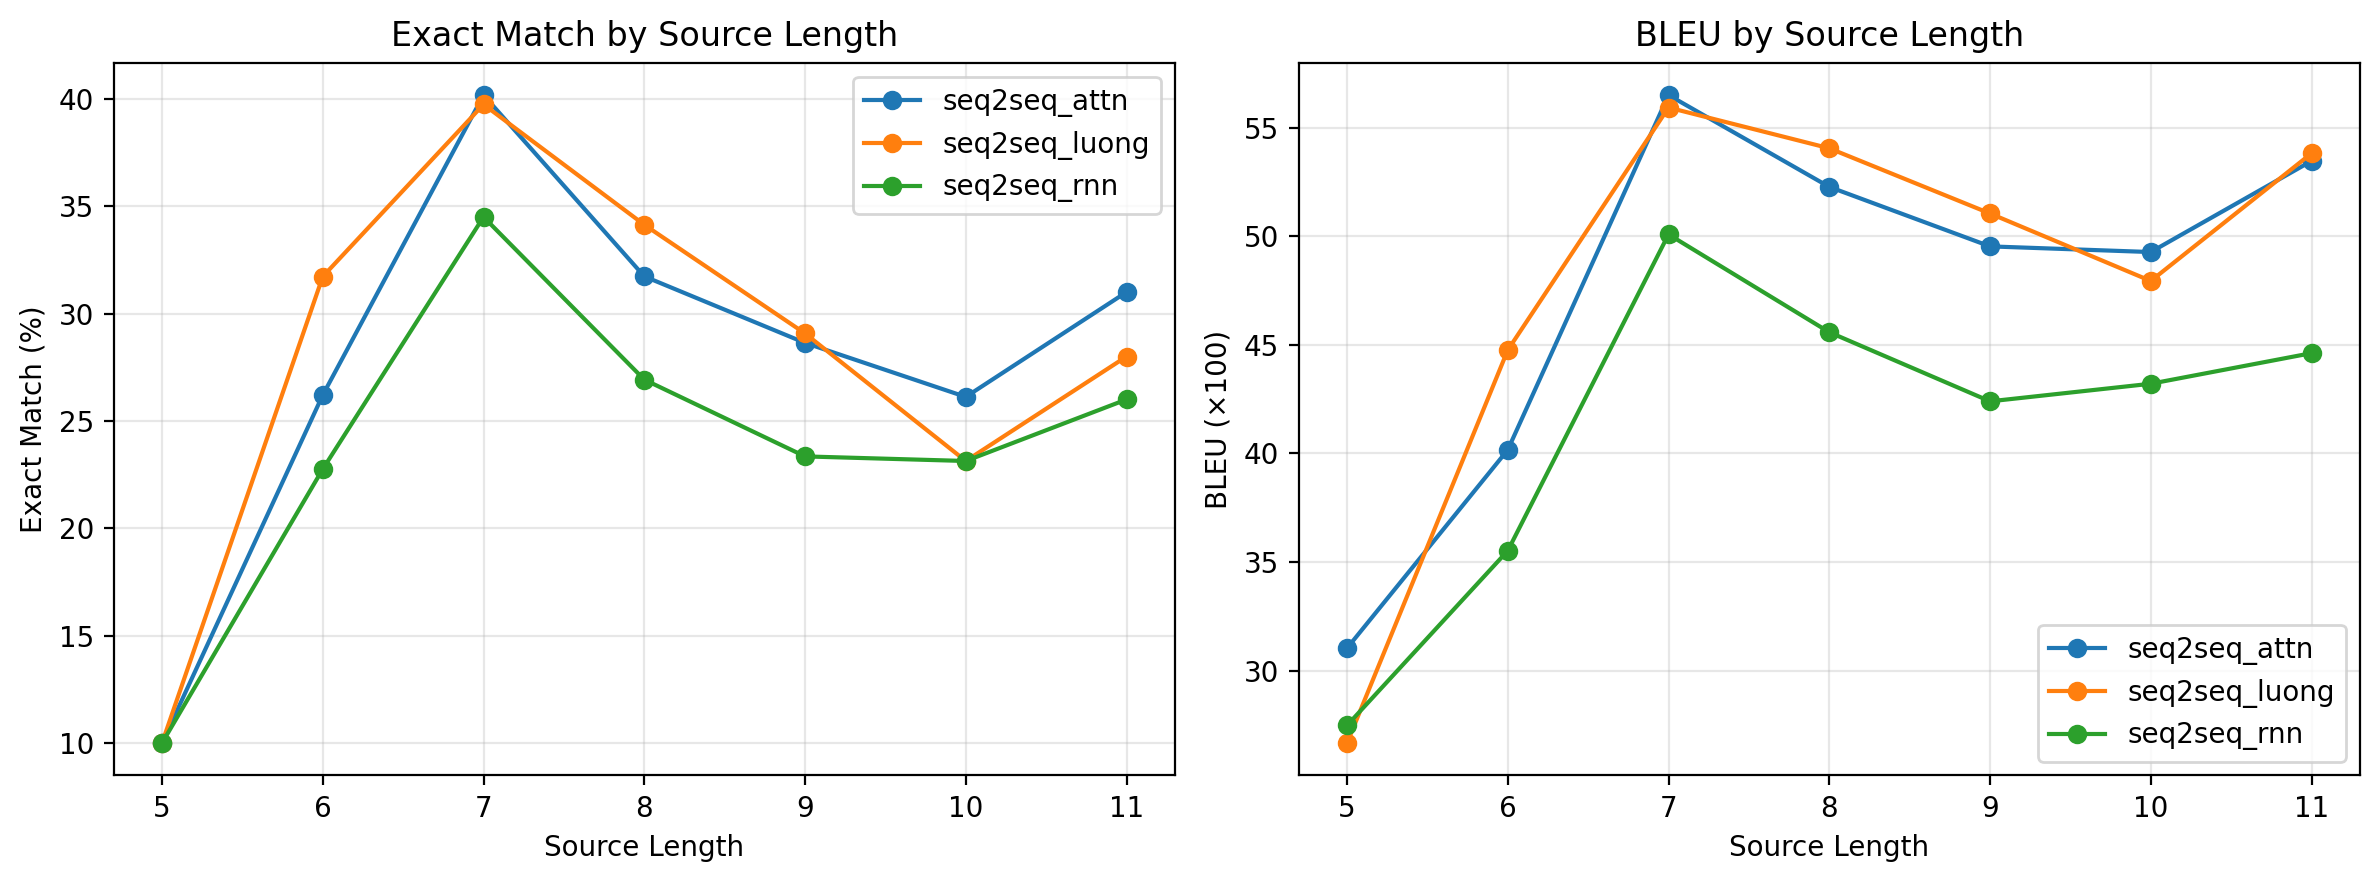
\includegraphics[width=0.95\textwidth]{fig/generated/lengthwise_line_plot.png}
    \caption{按真实输入长度统计的 Exact Match 与 BLEU 曲线}
    \label{fig:lengthwise_plot}
\end{figure}

从图\ref{fig:lengthwise_plot} 可以看出，测试集中的句长主要分布在 5 到 11 之间。随着输入句长增加，纯 RNN 基线整体更容易出现性能波动，而两种 attention 模型在多数长度点上都保持了更高的 Exact Match 与 BLEU。其中，Luong concat 与 Bahdanau 的整体曲线都明显高于纯 RNN，而 Luong concat 在多个长度点上略占优势。

为了便于从更粗粒度角度概括趋势，仍保留长度分桶统计结果。这里将测试样本分为 4--6、7--9 和 10--11 三个区间，对应样本数分别为 155、664 和 234。表\ref{tab:length_bucket} 进一步给出了各模型在不同区间上的 Exact Match 与 BLEU。

\begin{table}[H]
    \centering
    \scriptsize
    \setlength{\tabcolsep}{4pt}
    \resizebox{\textwidth}{!}{
    \begin{tabular}{lcccccc}
    \toprule
    \multirow{2}{*}{模型} & \multicolumn{3}{c}{Exact Match/\%} & \multicolumn{3}{c}{BLEU($\times 100$)} \\
    \cmidrule(lr){2-4}\cmidrule(lr){5-7}
     & 4--6 & 7--9 & 10--11 & 4--6 & 7--9 & 10--11 \\
    \midrule
    Seq2Seq-RNN & 21.94 & 28.31 & 24.36 & 34.74 & 45.59 & 43.86 \\
    Seq2Seq-Bahdanau & 25.16 \textcolor{green!50!black}{(+3.23)} & 33.58 \textcolor{green!50!black}{(+5.27)} & \textbf{28.21} \textcolor{green!50!black}{(+3.85)} & 39.36 \textcolor{green!50!black}{(+4.62)} & 52.36 \textcolor{green!50!black}{(+6.77)} & \textbf{51.09} \textcolor{green!50!black}{(+7.23)} \\
    Seq2Seq-Luong & \textbf{30.32} \textcolor{green!50!black}{(+8.39)} & \textbf{34.34} \textcolor{green!50!black}{(+6.02)} & 25.21 \textcolor{green!50!black}{(+0.85)} & \textbf{43.42} \textcolor{green!50!black}{(+8.68)} & \textbf{53.36} \textcolor{green!50!black}{(+7.77)} & 50.50 \textcolor{green!50!black}{(+6.64)} \\
    \bottomrule
    \end{tabular}
    }
    \caption{不同句长区间下的测试表现}
    \label{tab:length_bucket}
\end{table}

可以看到，在三个长度区间中，Luong concat 与 Bahdanau 都明显优于纯 RNN；其中在 4--6 和 7--9 区间，Luong concat 的指标更高，而在 10--11 区间，Bahdanau 的 Exact Match 与 BLEU 略占优势。这与逐长度折线图反映出的总体趋势是一致，说明加入注意力机制之后，模型能够更有效地利用输入序列中的对齐信息，因而在不同长度样本上都能获得更稳定的翻译效果。

% \begin{figure}[H]
%     \centering
%     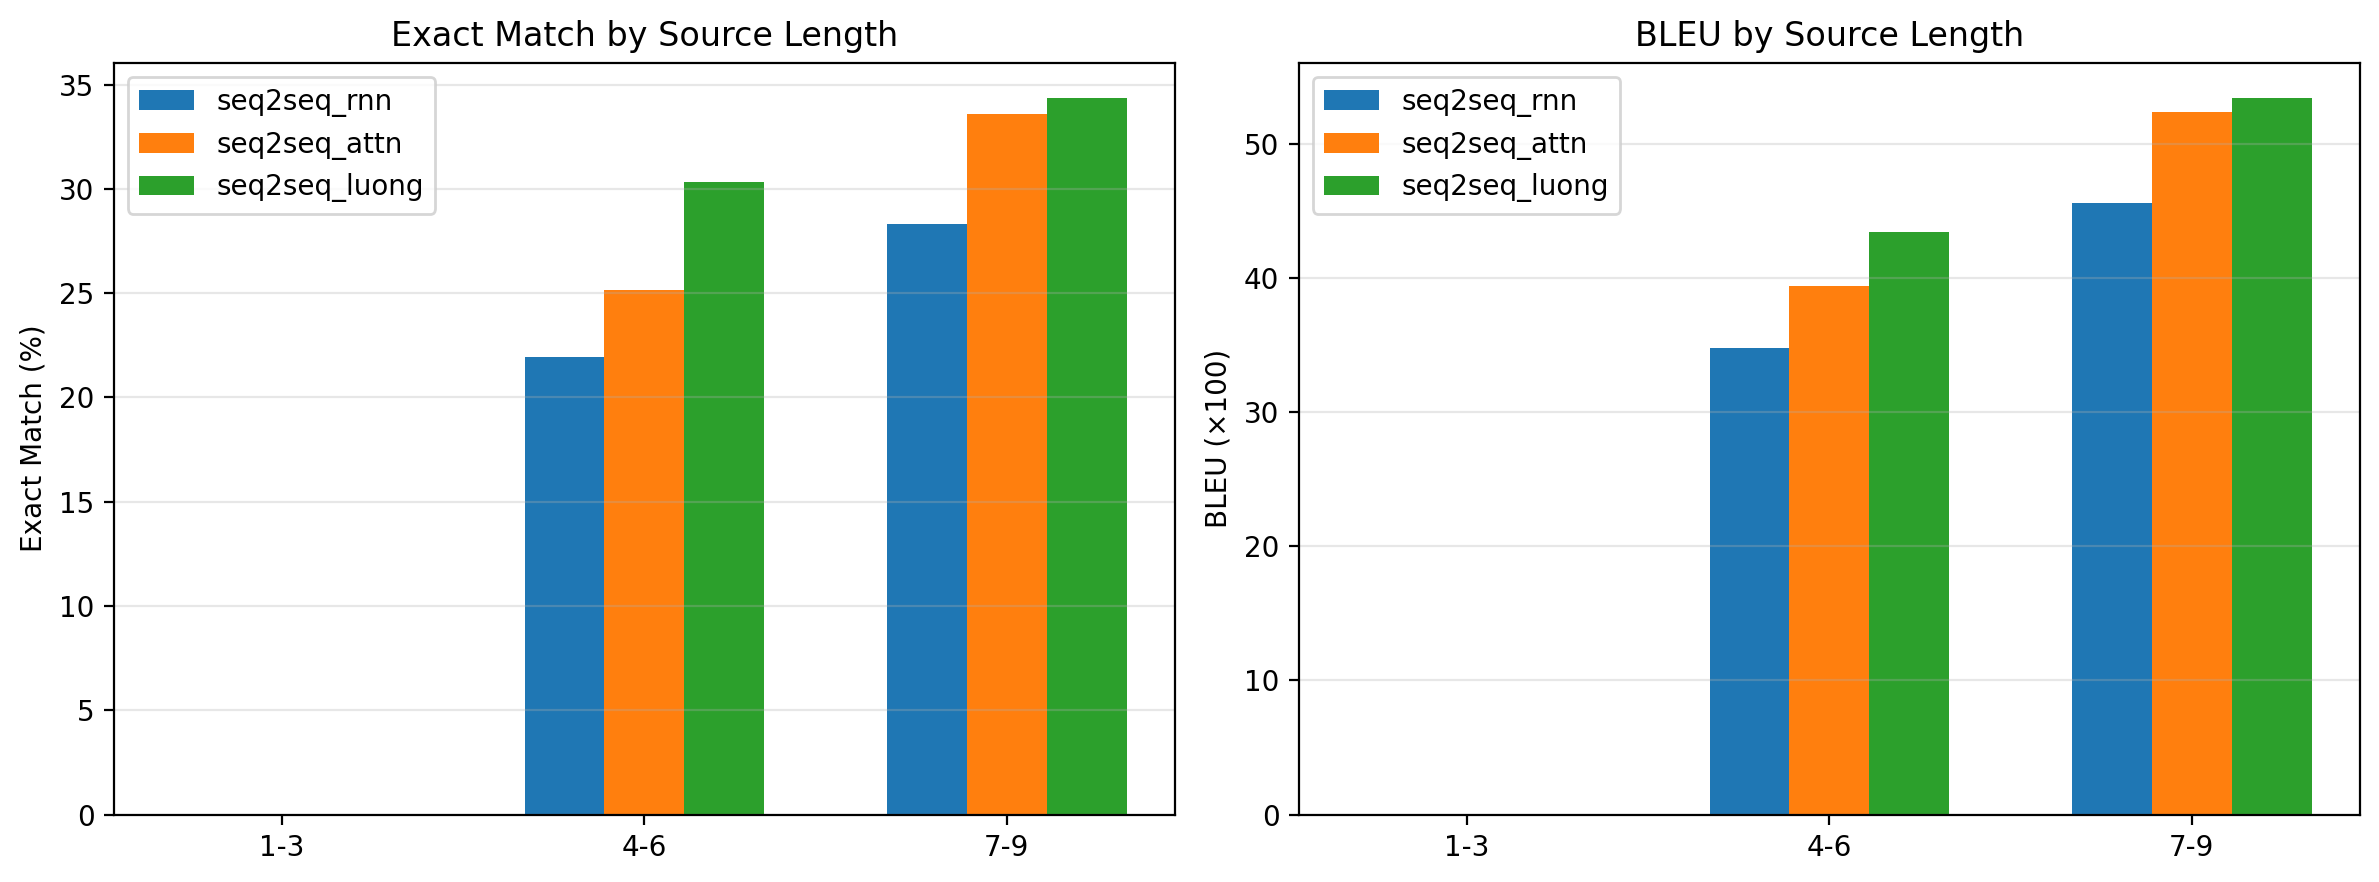
\includegraphics[width=0.9\textwidth]{fig/generated/length_bucket_comparison.png}
%     \caption{不同句长区间下的 Exact Match 与 BLEU 对比}
%     \label{fig:length_bucket_plot}
% \end{figure}

\subsection{注意力可视化分析}
对于带注意力机制的模型，除了比较最终翻译结果之外，还可以通过注意力热力图观察解码过程中源端与目标端之间的对齐关系。图\ref{fig:attn_vis} 展示了 Bahdanau 与 Luong 两种模型在测试样例上的注意力可视化结果。纯 RNN Seq2Seq 由于没有显式注意力权重，因此无法给出同类热力图。

从图\ref{fig:attn_vis} 可以看到，两种注意力模型在同一句法语样例上都会重点关注输入中的局部位置，因此具备一定的显式对齐能力。对于句子 \textit{elle a cinq ans de moins que moi .}，Bahdanau 模型生成了 \textit{she's five years younger than i am .}，Luong concat 模型生成了 \textit{she's five years younger than me .}，两者都较好完成了翻译，但注意力分布形态并不完全相同。具体来看，在生成 \textit{five years younger} 这一短语时，两种模型都把较高权重分配给源句中的 \textit{cinq ans de moins}，说明模型已经学到了较清晰的局部对齐关系；在生成句尾的 \textit{me / i am} 时，注意力又集中到 \textit{moi} 附近，表明模型能够识别法语代词与英语尾部成分之间的对应关系。相比之下，Bahdanau 的热力图分布相对更平滑一些，而 Luong concat 的响应位置更集中、峰值更尖锐，因此在该样例上表现出更强的局部聚焦特征。

\begin{figure}[H]
    \centering
    \subfigure[Bahdanau attention]{
        
\includegraphics[width=0.47\textwidth]{../outputs512/seq2seq_attn/final_seq2seq_attn_b512_e200/attention_examples/attention_02.png}
    }
    \subfigure[Luong attention (concat)]{
        
\includegraphics[width=0.47\textwidth]{../outputs512/seq2seq_luong_concat/sweep_seq2seq_luong_concat_optadam_h128_lr0p002_bs512/attention_examples/attention_02.png}
    }
    \caption{Bahdanau 与 Luong 模型在同一样例上的注意力热力图示例}
    \label{fig:attn_vis}
\end{figure}

\subsection{扩展实验：Scheduled Sampling}
在两种 attention 模型基础上，进一步加入 Scheduled Sampling，结果如表\ref{tab:ss_results} 所示。

\begin{table}[H]
    \centering
    \begin{tabular}{lccccc}
    \toprule
    模型 & Best Val Acc/\% & Test Acc/\% & Test Exact/\% & Test BLEU($\times 100$) \\
    \midrule
    Bahdanau & 73.09 & 71.87 & 31.15 & 51.08 \\
    Bahdanau + SS & 73.37 & 72.22 & 31.72 & 51.43 \\
    Luong (concat) & 73.99 & 72.73 & 31.72 & 51.77 \\
    Luong (concat) + SS & \textbf{74.62} & \textbf{73.41} & \textbf{31.91} & \textbf{51.89} \\
    \bottomrule
    \end{tabular}
    \caption{Scheduled Sampling 扩展实验结果}
    \label{tab:ss_results}
\end{table}

结果表明，Scheduled Sampling 在当前设置下总体带来了稳定但幅度有限的收益。对于 Bahdanau attention 和 Luongattention，加入 Scheduled Sampling 后，验证集最佳准确率、测试集 token accuracy、exact match 和 BLEU 均有小幅提升。由此可以认为，在当前短句翻译任务和数据规模下，Scheduled Sampling 确实具有一定帮助，但其影响仍明显弱于“是否加入注意力机制”这一因素本身。但也很有可能是在当下任务设置不太明显，因为主实验设置已经有0.5的概率输入真答案。



\subsection{扩展实验：Luong 不同打分方法比较}
为了进一步分析 Luong attention 内部打分函数的影响，又比较了 \texttt{dot}、\texttt{general} 和 \texttt{concat} 三种 scoring method 的结果。三者均采用与主实验一致的训练配置，并分别通过验证集准确率选择最优学习率，结果如表\ref{tab:luong_variants} 所示。

\begin{table}[H]
    \centering
    \small
    \resizebox{0.9\textwidth}{!}{
    \begin{tabular}{lccccc}
    \toprule
    打分方式 & 学习率 & Best Val Acc/\% & Test Acc/\% & Test Exact/\% & Test BLEU($\times 100$) \\
    \midrule
    dot & 0.003 & 72.35 & 71.20 & 31.05 & 49.91 \\
    general & 0.001 & 71.13 & 70.91 & 29.72 & 48.52 \\
    concat & 0.002 & \textbf{73.99} & \textbf{72.73} & \textbf{31.72} & \textbf{51.77} \\
    \bottomrule
    \end{tabular}
    }
    \caption{Luong attention 不同打分方法的结果比较}
    \label{tab:luong_variants}
\end{table}

从表\ref{tab:luong_variants} 可以看出，三种打分方式之间确实存在较明显差异。其中 \texttt{general} 版本整体最弱，而 \texttt{concat} 版本在验证集准确率、测试集 token accuracy、exact match 和 BLEU 上都取得了最好的结果，说明在当前任务上，更强的非线性匹配形式有助于改善 Luong attention 的对齐效果。

\subsection{为什么注意力机制有效}
结合前面的实验结果可以更直观地理解注意力机制为什么有效。主实验中，两种注意力模型在 Test Acc、Test Exact 和 BLEU 上都明显优于纯 RNN 基线；长度分析又表明，随着输入句长增加，纯 RNN 的性能波动更明显，而 Bahdanau 与 Luong 在多数长度点上都能保持更高的分数。这说明仅依赖编码器最终隐藏状态的做法，确实容易在句子稍长时受到信息压缩瓶颈的影响，而注意力机制通过在每个解码步重新利用编码器输出，减轻了这种固定长度表示带来的信息损失。

注意力热力图进一步解释了这种提升的来源。在同一样例上，Bahdanau 与 Luong 都能够把较高权重分配给与当前目标词最相关的源端位置，说明模型已经学到了较清晰的局部对齐关系。也正因为解码器可以按需“回看”输入序列，模型在生成关键短语和句尾成分时不必完全依赖单一上下文向量，从而更容易得到更稳定、更准确的翻译结果。因此，从最终指标、长度变化趋势以及可视化结果三个角度看，注意力机制的有效性都得到了比较一致的验证。

\subsection{Bahdanau 与 Luong 的差异}
结合前面的主实验结果可以看出，Bahdanau 与 Luong 两种注意力机制都明显优于纯 RNN 基线，说明无论采用加性还是乘性对齐，只要允许解码器在每一步重新利用编码器输出，都能够有效缓解固定上下文向量带来的信息瓶颈。不过在当前任务上，两者仍表现出一定差异：Bahdanau 模型整体较稳定，而采用 \texttt{concat} scoring 的 Luong 版本在 Test Acc、Test Exact 和 BLEU 上略优于 Bahdanau，说明乘性注意力在合适的打分方式下能够进一步提升最终效果。

这一点也与前面的注意力热力图和 Luong 打分方式比较结果相互印证。热力图显示，Bahdanau 的注意力分布相对更平滑，而 Luong concat 的响应位置更集中；在 \texttt{dot}、\texttt{general} 和 \texttt{concat} 的补充实验中，\texttt{concat} 版本又明显优于另外两种打分方式。所以，在具体的对齐打分设计上，这也会进一步影响模型的翻译表现。

\section{实验心得}
通过这次实验，可以比较清楚地体会到 Seq2Seq 模型从“固定上下文向量”到“显式注意力对齐”的差异。纯 RNN Seq2Seq 虽然结构最简单、训练开销也较小，但它需要把整句输入压缩到单个隐藏状态中，因此一旦句子变长，模型就更容易出现信息表达不足的问题。无论是主实验中的整体指标，还是按句长统计的结果，都表明加入注意力机制之后，模型在翻译质量和稳定性上都有明显改善，这使得“注意力为什么重要”不再只是理论上的描述，而是能够从实验结果中直接观察出来。

在两类注意力模型中，Bahdanau 与 Luong 都取得了比纯 RNN 更好的结果，但它们的差异也说明，注意力机制本身并不是一个单一组件，具体的对齐打分设计会进一步影响模型效果。当前实验中，Luong 分支中的 \texttt{concat} 版本在主实验和补充实验中都表现最好，说明在这个短句翻译任务上，更强的非线性匹配形式确实带来了收益；而注意力热力图又展示出 Bahdanau 分布更平滑、Luong concat 聚焦更集中的特点，使模型结构差异与可视化现象能够对应起来。

另外，这次实验也让我学到 teacher forcing 的思想。它并不是简单地“喂给模型正确答案”，而是在训练阶段有控制地改变解码器下一步所接收的输入来源，使模型一部分时间依赖真实目标词，另一部分时间依赖自身预测结果。从这个角度看，它与 dropout 在思想上有一定相似性，即都通过在训练过程中引入随机扰动，避免模型过度依赖某一种固定的信息路径；不过两者的作用位置并不相同，dropout 主要作用于网络内部表示，而 teacher forcing 调整的是序列生成时的输入方式。这种训练与推理口径差异的问题，也让我更容易理解为什么后续论文中还会引出 Scheduled Sampling 这样的改进策略。

\newpage
\appendix
\section{代码目录说明}
为便于查阅与提交，本实验的关键代码已经统一整理到 \texttt{final/code/} 目录下，最终报告 PDF 放在 \texttt{final/report.pdf}。若需要快速定位核心实现，可优先查看以下文件：
\begin{itemize}
    \item \texttt{final/code/train.py}：单次正式训练入口；
    \item \texttt{final/code/sweep\_lr.py}：学习率搜索入口；
    \item \texttt{final/code/src/models/seq2seq\_rnn.py}：纯 RNN Seq2Seq；
    \item \texttt{final/code/src/models/seq2seq\_attn.py}：Bahdanau attention；
    \item \texttt{final/code/src/models/seq2seq\_luong.py}：Luong attention 与不同 scoring method；
    \item \texttt{final/code/src/engine.py}：训练、验证、测试以及 BLEU 统计；
    \item \texttt{final/code/scripts/generate\_report\_assets.py}：报告图表与表格生成；
    \item \texttt{final/code/model\_prints/}：三种主模型的结构打印结果。
\end{itemize}

\bibliographystyle{plain}
\bibliography{reference.bib}

\end{document}
